\documentclass{article}

\usepackage{float}
\usepackage{graphicx}
\usepackage{dirtytalk}

\author{Abdelsalam ElTamawy\\900170376}
\title{Assignment 3}

\begin{document}

\maketitle

\section{Data processing}

No major data processing was used beyond resizing the images so they all are the same size. Other forms of data processing were also attempted such at adjusting saturation and adding sharpness but none proved to have a meaningful improvement on the results. As for what the size was set to upon resizing the images, 32*32 proved to give a nice medium between performance, memory consumption and accuracy.

\section{Hyper parameters}

As with the last assignment, All hyper parameters started with their \say{rule of thumb} and then dialed in to their final values.

As for the network architecture of the model, the fully connected section remained unchanged from the first assignment at 2 layers with 1200 nodes each since it proved to perform so well the last time.

After trying a handful of configuration for the convolutional layers. I ended up settling on having alternating convolving and max pooling layers. The choosing the configuration of the convolving layers centered around the philosophy of making the volume produced at each layer be smaller along the cross section and deeper, providing room to draw features from nicely.

Step sizes were kept rather small since the data already was at a small 32*32.
Max pooling layers were kept at smaller size as well, also so we don't have too few features to draw from at the fully connected layers.

After some experimentation, the convolving layers ended up having the following configuration:
\begin{enumerate}
	\item 3*3 convolution kernel, padding 2, 4 filters, step size of 1.
	\item 2*2 max pooling, step size of 2.
	\item 500 node fully connected layer.
	\item 500 node fully connected layer.
	\item 5 node classification layer.
\end{enumerate}

Now that the most critical hyper parameter is settled, we can now tune the other hyper parameters.
Similar to last time, I defined a set of limits at which each parameter would give NaN results and then logarithmically randomly generate values for each hyper parameter on this scale.

Then to dial it in further, we randomly generate all parameters according to this smaller region recommended to us by the previous set of graphs.

\begin{figure}[H]
	\centering
	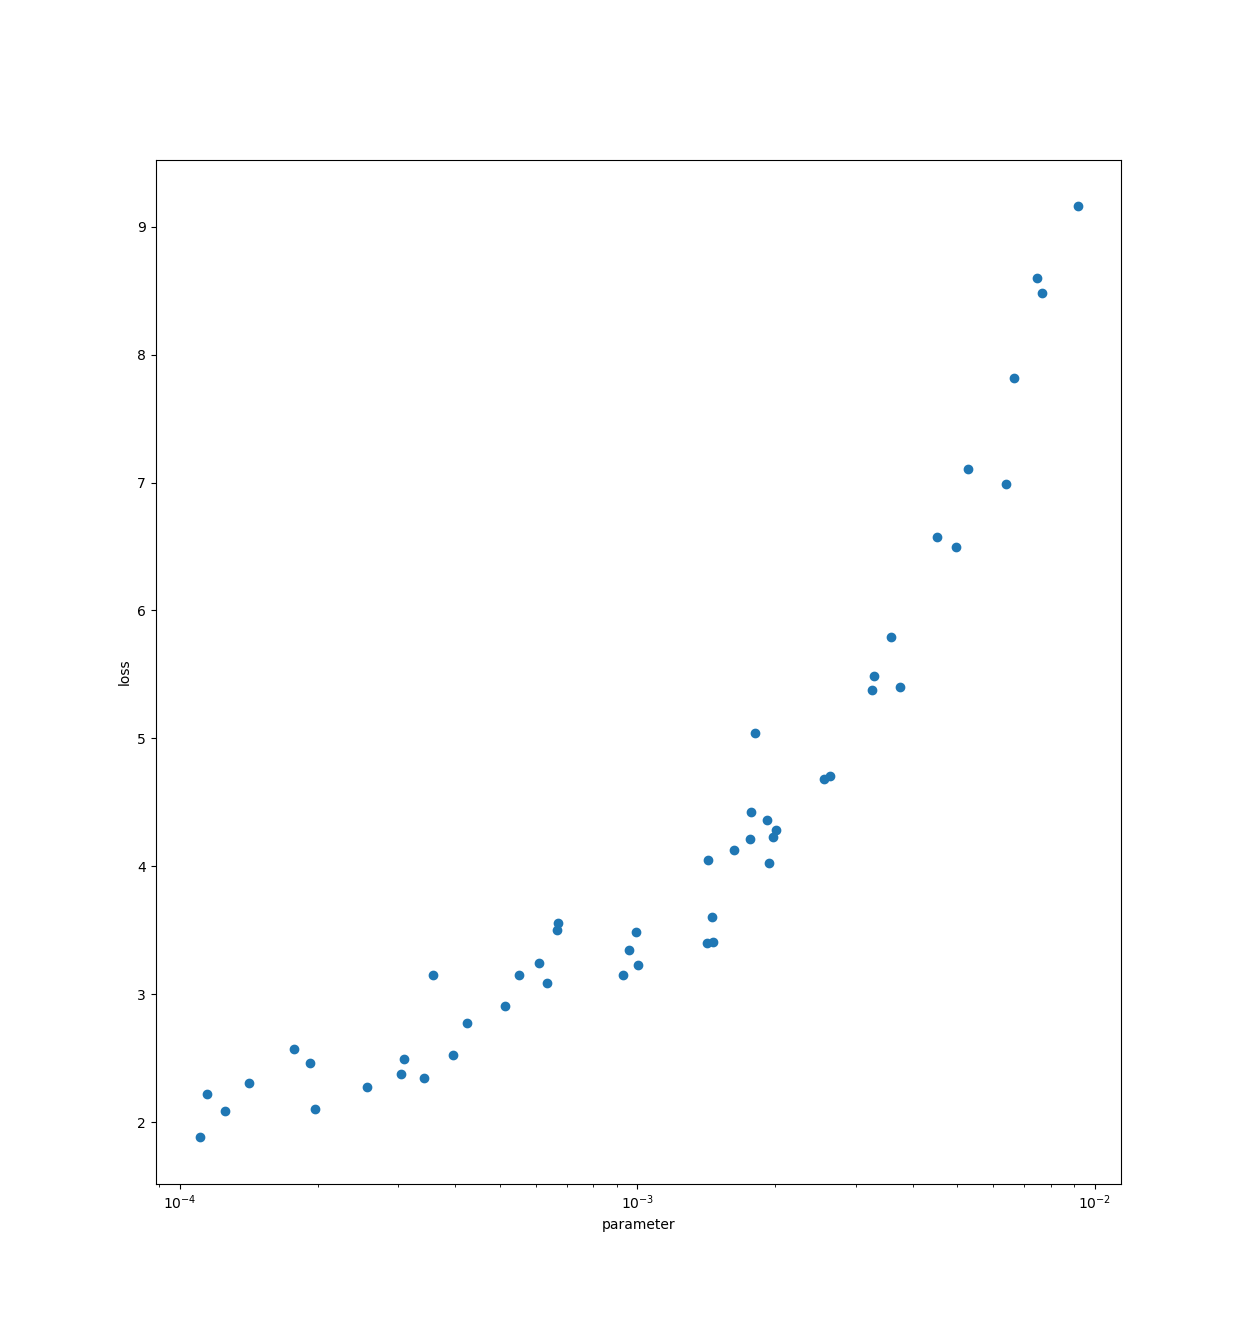
\includegraphics[width=\textwidth]{reg.png}
	\caption{Tuning for regularization}
\end{figure}

\begin{figure}[H]
	\centering
	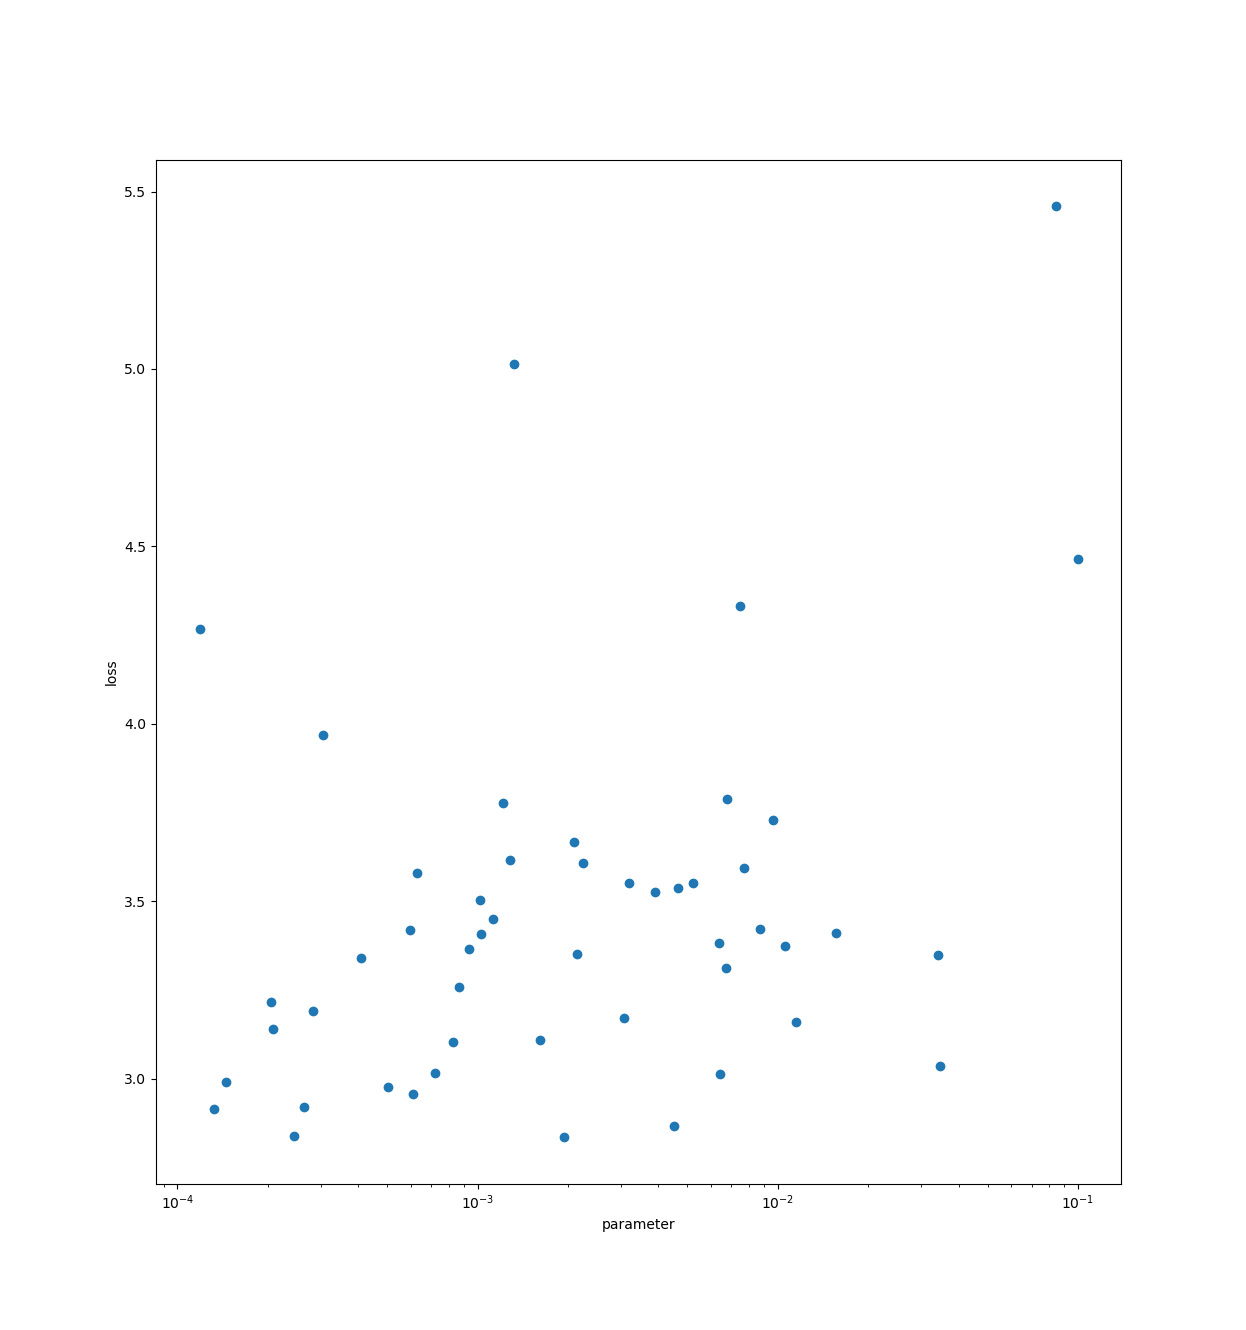
\includegraphics[width=\textwidth]{leaky.png}
	\caption{Tuning for leaky RELU factor}
\end{figure}

\begin{figure}[H]
	\centering
	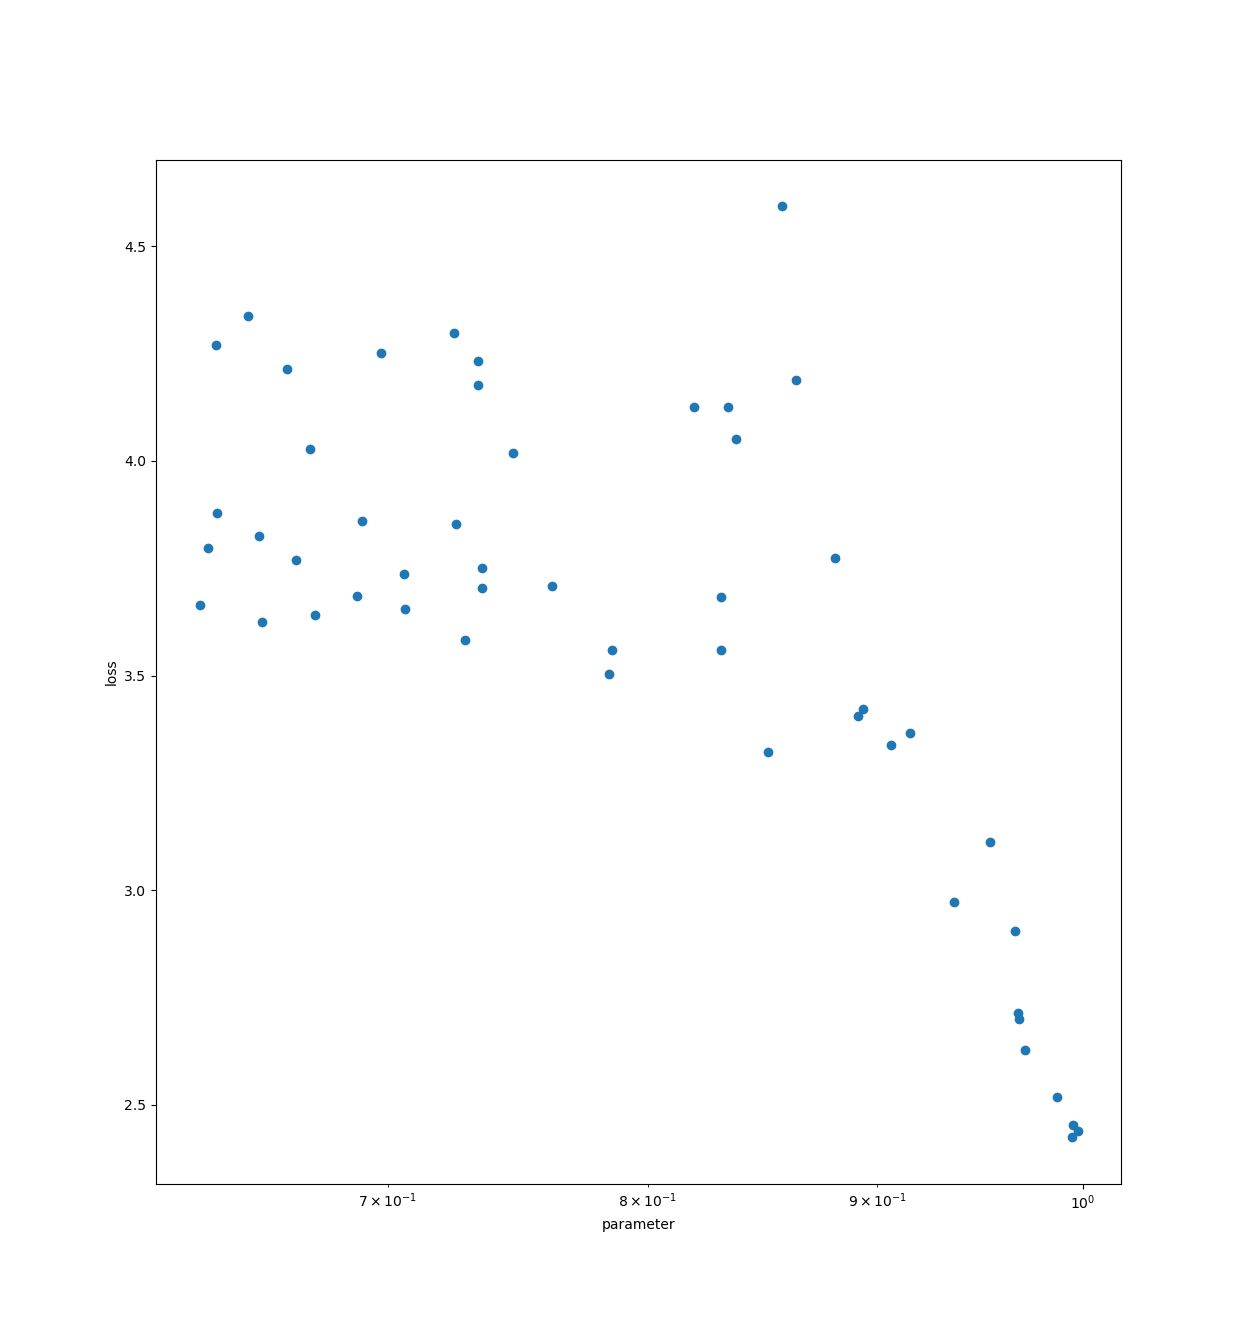
\includegraphics[width=\textwidth]{mom.png}
	\caption{Tuning for momentum}
\end{figure}

\begin{figure}[H]
	\centering
	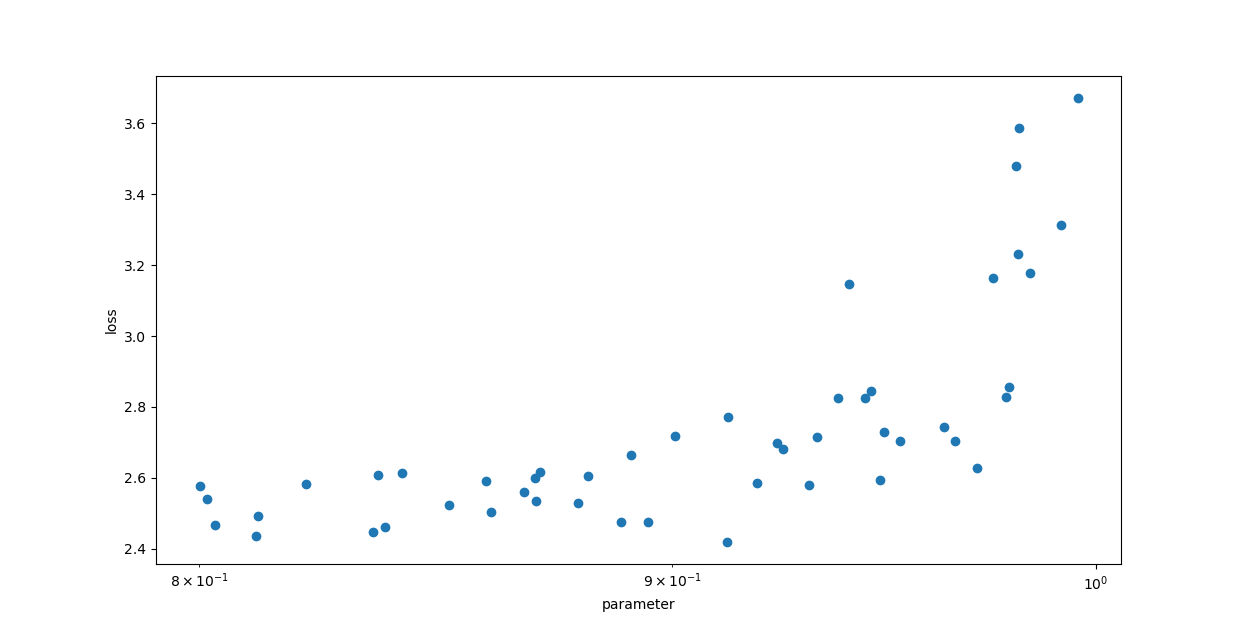
\includegraphics[width=\textwidth]{accu.png}
	\caption{Tuning for accumulator}
\end{figure}

\begin{figure}[H]
	\centering
	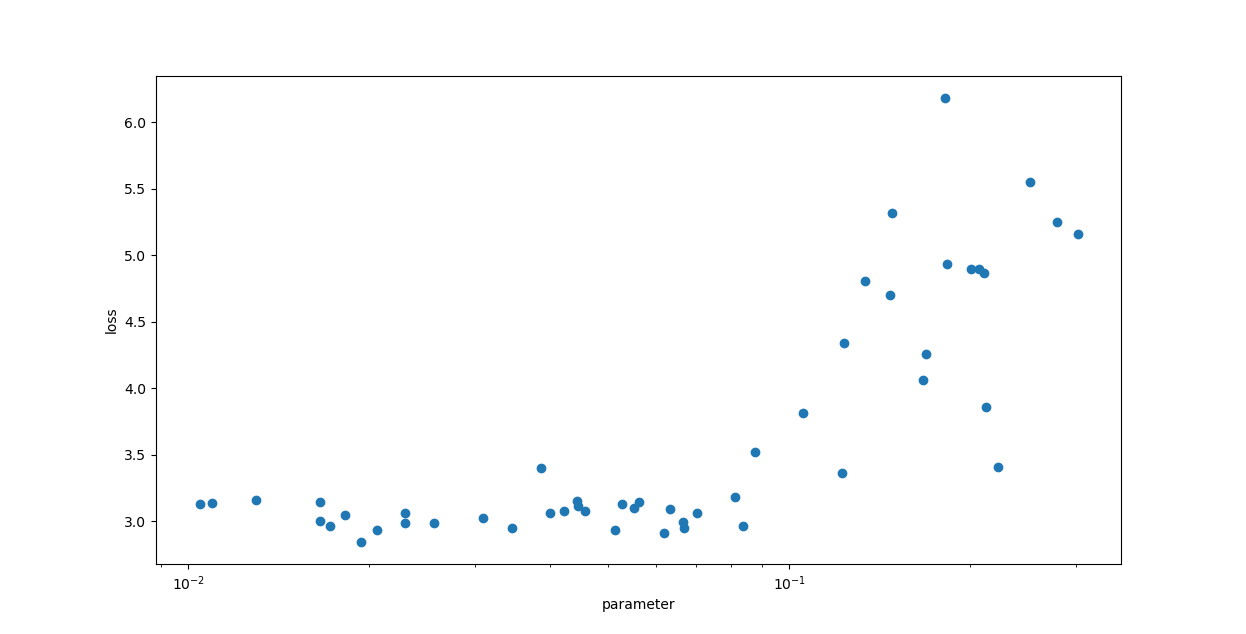
\includegraphics[width=\textwidth]{drop.png}
	\caption{Tuning for drop rate}
\end{figure}

\section{Training and losses}

Seed used is 42.

\begin{figure}[H]
	\centering
	\includegraphics[width=\textwidth]{train.png}
\end{figure}

\section{Comparison}

\begin{figure}[H]
	\centering
	\includegraphics[width=\textwidth]{figure_6.png}
	\caption{Per class results of training}
\end{figure}

The jump from KNN to NN was for the most part a direct almost constant increase across the board for the accuracy of all flowers.
CNN on the other hand, seems to sort of \say{normalize} the results more, as in there is less of a direct constant relation from the results from KNN and NN to CNN, the lower scoring flowers had a marked increase. This suggests there being more \say{reasoning} happening behind CNN as it really is with it's convolutions.

\section{ACCR}

A final ACCR of 60.2\% after almost 3000 epochs.

\begin{figure}[H]
	\centering
	\includegraphics[width=\textwidth]{figure_5.png}
\end{figure}

Stopped at that point since the accuracy seems to level out and due to time constants.

\end{document}
